\documentclass[handout]{beamer}
\usetheme{Madrid}
\usepackage{pdfpages}
\usepackage[utf8x]{inputenc}
\usepackage{url}
\usepackage{graphicx}
\usepackage{graphics}
\usepackage{adjustbox}
\usepackage{ragged2e}
\usepackage{amsmath, amssymb}
\usepackage{verbatim}
\usepackage{soul}
\usepackage{textpos}
\usepackage{xcolor}
\usepackage{tcolorbox}
\usepackage{lmodern,textcomp}
 \setbeamertemplate{enumerate items}[default]
 \setbeamertemplate{itemize items}[circle]
 \setbeamertemplate{frametitle continuation}{}
\setbeamertemplate{section in toc}[circle]
\setbeamertemplate{subsection in toc}[circle]

\usepackage{tabulary, booktabs}

\usepackage{hyperref}
\hypersetup{
    colorlinks=cyan,
    linkcolor=true,
    filecolor=cyan,      
    urlcolor=cyan,
}

\beamertemplatenavigationsymbolsempty

%%%%%%%%%%%%%%%Color%%%%%%%%%%%%%%%
\definecolor{KIPlum}{HTML}{880052}
\definecolor{box}{RGB}{250, 117, 144}
\usecolortheme[named=KIPlum]{structure}

%%%%%%%%%%%%%%%Bibliography setting%%%%%%%%%%%%%%%
\usepackage[numbers,comma,sort&compress]{natbib}
\makeatletter
\renewcommand{\@biblabel}[1]{#1.} %remove brackets from the ref list
\makeatother




%%%%%%%%%%%%%%%Title page%%%%%%%%%%%%%%%

\title[Applied Epi I: Data Management]{Applied Epidemiology I: Data Management}
\date{\today}
\author[Enoch Yi-Tung Chen]{Enoch Yi-Tung Chen}
\institute[MEB]{Department of Medical Epidemiology and Biostatistics, Karolinska Insitutet}

%%%%%%%%%%%%%%\begin{document}%%%%%%%%%%%%%%%%

\begin{document}

\begin{frame}
\maketitle 
\end{frame}

%%%%%%%%%%%%%%Outline%%%%%%%%%%%%%%%%
\begin{frame}{Acknowledgements}
This course material in data management is based on my learning from \href{https://staff.ki.se/people/annajo}{Anna Johansson}'s \href{https://play.ki.se/media/Data+Management+and+research+documentation+for+researchers/0_h64ki6v7?_ga=2.131118287.1557257458.1589785892-1364153581.1557067020}{workshop at KI library}\footnote{This workshop is currently available on KI Play as well. }, teachings in \href{https://kiwas.ki.se/katalog/katalog/kurs/851;jsessionid=e42ee2c1f6b081f28bf83e3d0321?lang=en}{Good Data Management Practice in Epidemiological Research}, and MEB Guidelines for Documentation and Archiving Version 6 \footnote{The Department of Medical Epidemiology and Biostatistics, Karolinska Institutet. MEB Guidelines for Documentation and Archiving Version 6. 2018.}. I personally want to thank for their effort on education in data management.

I especially want to thank Marlene Stratmann for reviewing the slides and Prof. Paul Dickman for providing me with suggestions to improving the teaching.

\end{frame}

%%%%%%%%%%%%%%Outline%%%%%%%%%%%%%%%%
\section*{Outline}
\begin{frame}{Outline}
          \tableofcontents
\end{frame}

%%%%
\section{What if no data management?}

\begin{frame}{\secname}
In the beginning, 
\begin{center}
		
\includegraphics[scale=0.4]{image/desktop}
\end{center}
\end{frame}

\begin{frame}{\secname}
In the half-way of the research, \\
\begin{center}
		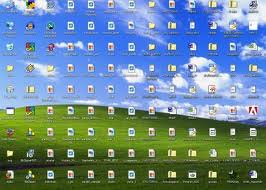
\includegraphics[scale=0.5]{image/messy-desktop}
\end{center}
\end{frame}

\begin{frame}{\secname}
At the end, or saying you cannot even walk till the end?

\begin{center}
		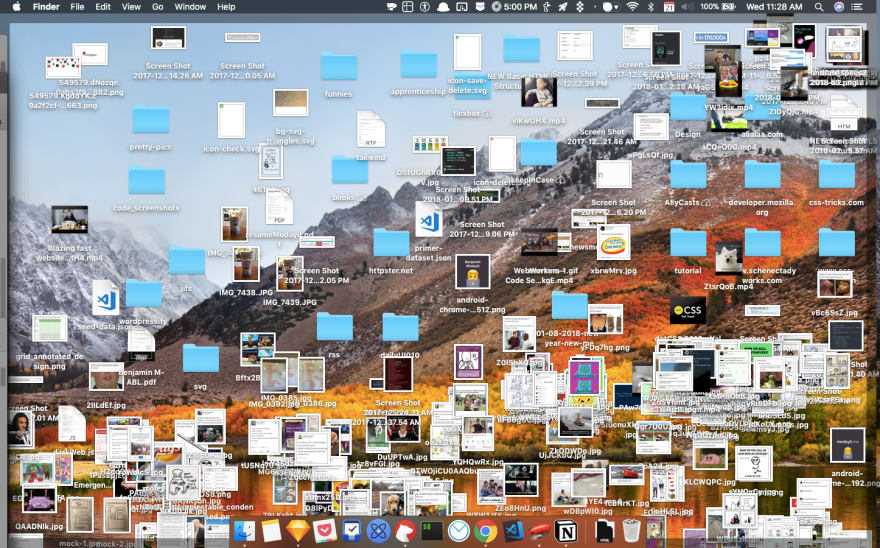
\includegraphics[scale=0.3]{image/more-messy-desktop}
\end{center}
\end{frame}

\begin{frame}{\secname}
Imagine now 
\begin{itemize}

	\item<1|handout:1-> if you want to correct Table I, where is the do file for descriptive analysis?
	\item<2|handout:2-> if your supervisor says, "Please summarise how far you've gone in this project." You probably cannot just drop him/her your syntax. 
	\item<3|handout:3-> if your classmate asks you to teach her how to write a certain Stata code, you remember you've done it before, but where did you put it?
	\item<4|handout:4> if your collaborator needs to take over your analysis, can he/she understand what you've completed?
\end{itemize}
\end{frame}

\begin{frame}{\secname}

\begin{center}
		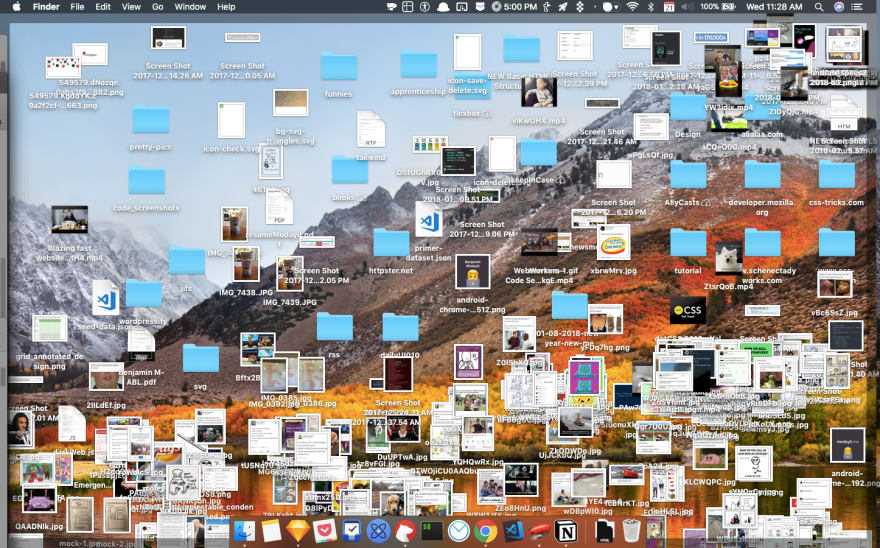
\includegraphics[scale=0.3]{image/more-messy-desktop}
\end{center}
\end{frame}

\begin{frame}{\secname}

So I would say you need to have a friend called \\
\begin{center}
	{\huge \textbf{Data Management}}
\end{center}

\end{frame}

%%%%
\section{Aims of data management (also learning outcomes)}
\begin{frame}{\secname}
\begin{itemize}
	\item<1|handout:1-> To ensure the analysis is reproducible
	\item<2|handout:2-> To work coherently and efficiently with yourself 
	\item<3|handout:3-> To ensure the project can be understood by others (supervisors, collaborators, and future readers)
	\item<4|handout:4> To create a good work flow and enhance accuracy of work 	
\end{itemize}
\end{frame}

%%%%
\section{Good folder structure}
\begin{frame}{Good folder structure}
	\begin{columns}
	\begin{column}{0.5\textwidth}
	The core elements of folders are listed below:
		\begin{itemize}
				\item Data
				\item Documents
				\item Log
				\item Output
				\item Program
		\end{itemize}
	\end{column}
	
	\begin{column}{0.5\textwidth}
	\begin{figure}
			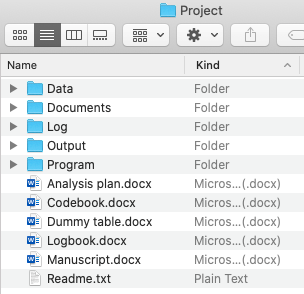
\includegraphics[scale=0.4]{image/structure}
			\caption{Good project folder structure. (Please bear with me that I am Mac user!)}
	\end{figure}
	\end{column}
	\end{columns}

\end{frame}

%%%%
\section{Good documents}
	\begin{frame}{Good documents}
	\begin{columns}
	\begin{column}{0.5\textwidth}
	Besides good folder structure, you should also consider keeping good documents
		\begin{itemize}
				\item Analysis plan
				\item Codebook\footnotemark
				\item Dummy table
				\item Logbook\footnotemark[\value{footnote}]
				\item Manuscript
		\end{itemize}
	
	\end{column}
	
	\begin{column}{0.5\textwidth}
	\begin{figure}
			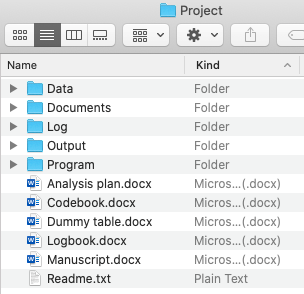
\includegraphics[scale=0.4]{image/structure}
			\caption{Good project folder structure.}
	\end{figure}
	\end{column}
	\end{columns}
	\footnotetext[3]{can be included in analysis plan as well}
\end{frame}

%%%%
\section{Good Readme.txt}	
\begin{frame}{Good Readme.txt}
\begin{columns}
	\begin{column}{0.5\textwidth} 
	\begin{itemize}
	\item You should illustrate how to use these documents/folders in the Readme.txt. 
	\item  A good Readme.txt is a good tourist guide in this project folder.

	\end{itemize}
	\end{column}
	
	\begin{column}{0.5\textwidth}
	\begin{figure}
			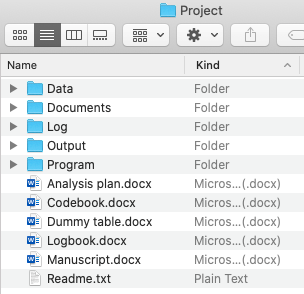
\includegraphics[scale=0.4]{image/structure}
			\caption{Good project folder structure.}
	\end{figure}
	\end{column}
	\end{columns}
\end{frame}

%%%%
\section{Good habits on coding}
\begin{frame}[allowframebreaks]{Good habit on coding}
\begin{columns}
	\begin{column}{0.3\textwidth} 
	\begin{itemize}
	\item log on
	\item[] 
	\item Filename
	\item Study
	\item Created
	\item Updated
	\item Purpose
	\item Note
	\item[] 
	\item \textbf{Start your code}
	\item[] 
	\item log close
	\end{itemize}
	\end{column}
	
	\begin{column}{0.7\textwidth} 
			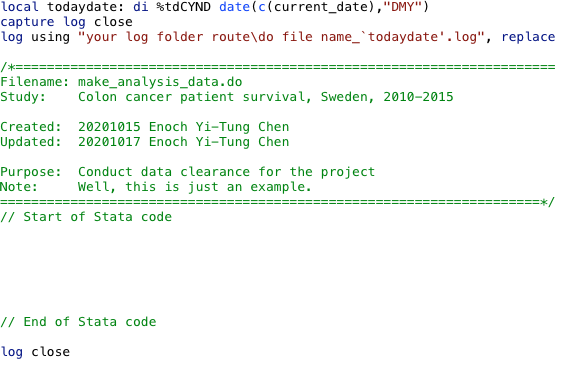
\includegraphics[scale=0.5]{image/header}
	\end{column}

\end{columns}

\newpage

\begin{itemize}
	\item Talk to yourself what you are doing.
	\item You've got a friend in me! (Parallel analysis)
	\item Rubber duck debugging
	\item[] 
	\item[]  \centering 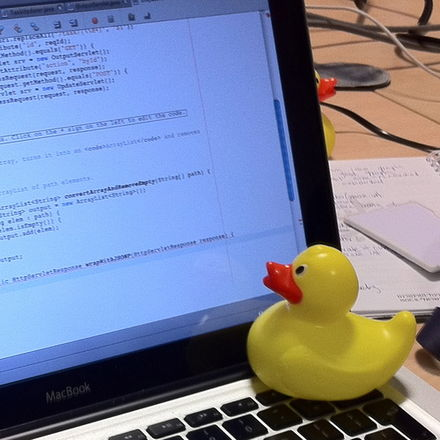
\includegraphics[scale=0.3]{image/rubberduck}
\end{itemize}

\end{frame}

%%%%
\section{Other do's and don'ts}

\begin{frame}{\secname}

\begin{enumerate}[<+->]
	\item<1|handout:1->  Use a shared drive. (Required to do that because of data privacy.)
	\item<2|handout:2->  Give appropriate names to your files and variables.
		\begin{itemize}[<+->]
			\item<3|handout:3->  No stupid names, such as new1, new2, new3, final1, final2, final3, latest1
			\item<4|handout:4->  No space in-between \& No special character (in case, the software cannot read.)
			\item<5|handout:5->  For binomial variables, $=1$ implies yes, and $=0$ implies no.
			\item<6|handout:6->  Label your variables, please!
		\end{itemize}
	\item<7|handout:7->  Same names for linking files (.do .r .sas $\rightarrow$ .log $\rightarrow$ .doc)
	\item<8|handout:8>  Don't replace the original files or variables. (Well if you accidentally do this, you still get a chance to revert if using shared drive.)
\end{enumerate}
	
\end{frame}

%%

\section{Wrap it up}
\begin{frame}{Wrap it up}
\begin{itemize}
\item<1|handout:1->  In summary, a good data management contains GOOD
\begin{enumerate}
	\item folder structure
	\item documents
	\item readme
	\item habits
\end{enumerate}

\item<2|handout:2>  How can this lecture help you? \\
\item<2|handout:2>  I attached the resources you can use for DM your current and future projects.
\end{itemize}
\end{frame}

\end{document}